\documentclass[8pt]{beamer}
\usepackage[utf8]{inputenc}
\usepackage{xcolor}
\usepackage{colortbl}
\usepackage{epsfig}
% \usepackage{cancel}
% \usepackage{ulem}
% \usepackage{threeparttable} % Joao Pela: 
\usepackage{amsmath}
\usepackage{hyperref}
% \usepackage{relsize}
% \usepackage{feynmp}         % For latex produced Feynman Diagrams

% Rule for feynmp diagrams to be considered graphics
\DeclareGraphicsRule{*}{mps}{*}{}

% New compile sequence for feynmp
\makeatletter
\def\endfmffile{%
  \fmfcmd{\p@rcent\space the end.^^J%
          end.^^J%
          endinput;}%
  \if@fmfio
    \immediate\closeout\@outfmf
  \fi
  \ifnum\pdfshellescape=\@ne
    \immediate\write18{mpost \thefmffile}%
  \fi}
\makeatother

\usetheme{Madrid}

\author[João Pela]{J. Pela}
\title[QCD Control]{Study on new possible variables to control QCD}
% \subtitle{PhD 3 Months Report}
\institute{Imperial College London}
\date{2013-06-17}

% The log drawn in the upper right corner.
\logo{\includegraphics[height=0.115\paperheight]{img/Logo_CMSICL.png}}

\begin{document}
\setlength{\unitlength}{1mm}

\begin{frame}
  \titlepage
\end{frame}

\begin{frame}{Introduction and Motivation}

\begin{block}{Control of QCD}
  
\begin{columns}
  
  \column[t]{5.5cm}
  QCD is a major concern of our analysis, and the search for ways to control/estimate it a priority.
  \begin{itemize}
    \item The current event selection only uses variables over the dijet system of the the MET.
    \item Charateristics of the Dijet+MET system can be exploited to reduce the QCD background 
    with minimal signal loss.
    \begin{itemize}
      \item Total energy of selected objects (2 jets and MET).
      \item Balance over MET and dijet system.
    \end{itemize}
  \end{itemize}
  
  \column[t]{5.5cm}
    \begin{center}
      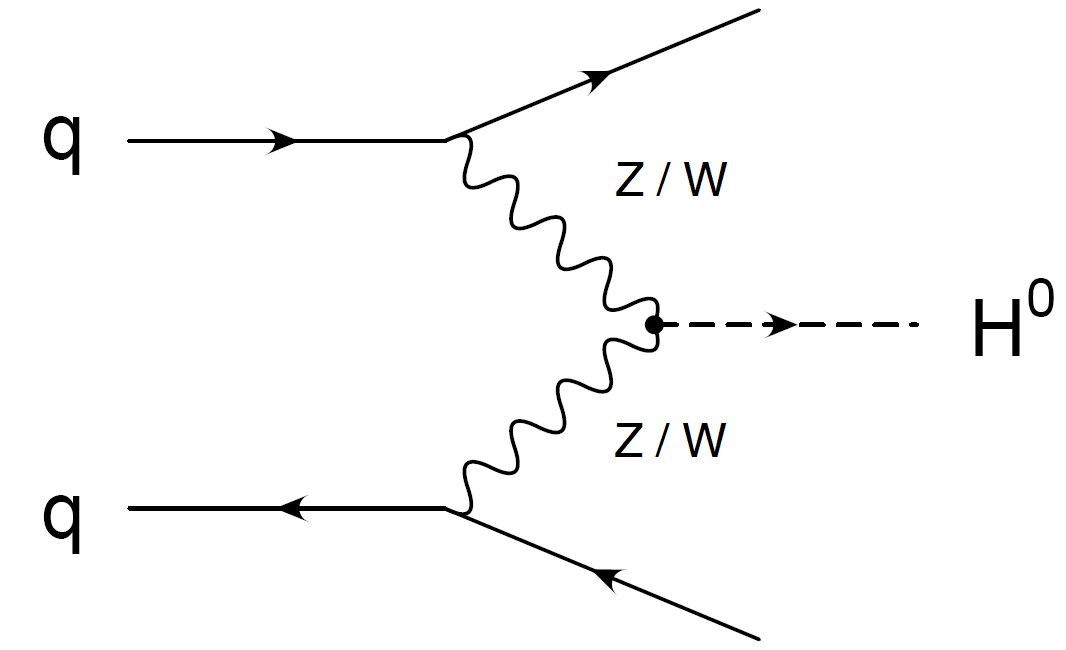
\includegraphics[width=1.00\textwidth]{img/vector_boson_fusion.PNG} 
    \end{center}
  
\end{columns}
  
\end{block}

\end{frame}

\begin{frame}{Definition of variables}
 
\begin{block}{Control of QCD}
  
  Three variable are being analyzed for possible use on this analysis
  \begin{itemize}
   \item Scalar Tri-Object Sum = $|pT(jet1)|+|pT(jet2)|+|MET|$
   \begin{itemize}
     \item Similar to HT
     \item The higher it is the better is average selected object resolution
   \end{itemize}
   \item Dijet pT fraction = $p_{T}(dijet)/(p_{T}(dijet)+MET)$
   \begin{itemize}
     \item Refects balance dijet+MET system
     \item Signal should be highly concentrated around 0.5
   \end{itemize}
   \item Vector Tri-Object Sum = $|Vector Sum(pT(jet1)+pT(jet2)+MET)|$ 
   \begin{itemize}
     \item Refects balance dijet+MET system
     \item Signal should be highly concentrated around zero
     \item Study underway to possibly include the jet and MET resolution in the variable 
   \end{itemize}
  \end{itemize} 
  
\end{block}

\end{frame}

\begin{frame}{Individual Variables after TightMjj}
 
\begin{block}{Scalar Tri-Object Sum}
 
\begin{columns}
 
\column[t]{5.5cm} 
\begin{itemize}
  \item Like expected this variable by itself will not allow a big signal discrimination but 
conjugated with other variables it may be helpful.
  \item It can have the same role that HT has in conjunction with alphaT in the SUSY analysis. 
\end{itemize}


\column[t]{5.5cm} 
  \begin{center}
  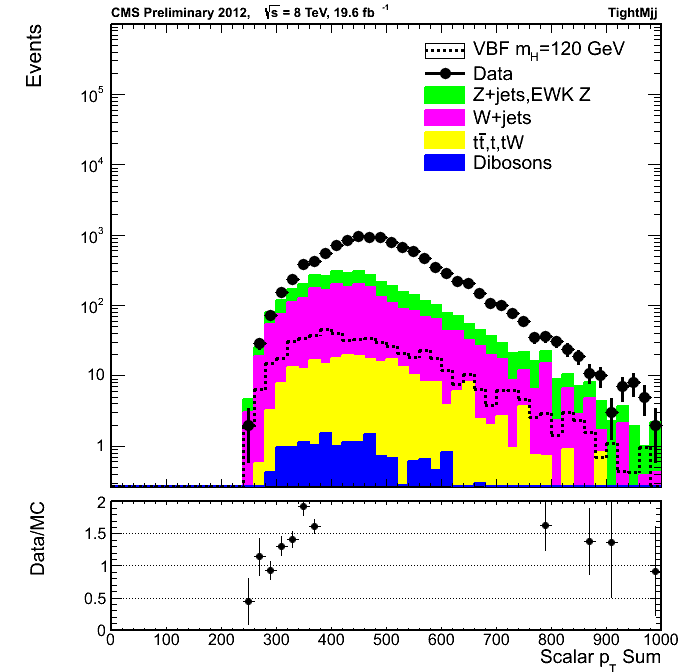
\includegraphics[width=1.00\textwidth]{img/htMET_2012_TightMjj_log.png}
  \end{center}
 
\end{columns}

\end{block}
 
\end{frame}

\begin{frame}{Individual Variables after TightMjj}

\begin{columns}

\column[t]{5.5cm}   
\begin{block}{After TightMjj cut}
 
  \begin{center}
  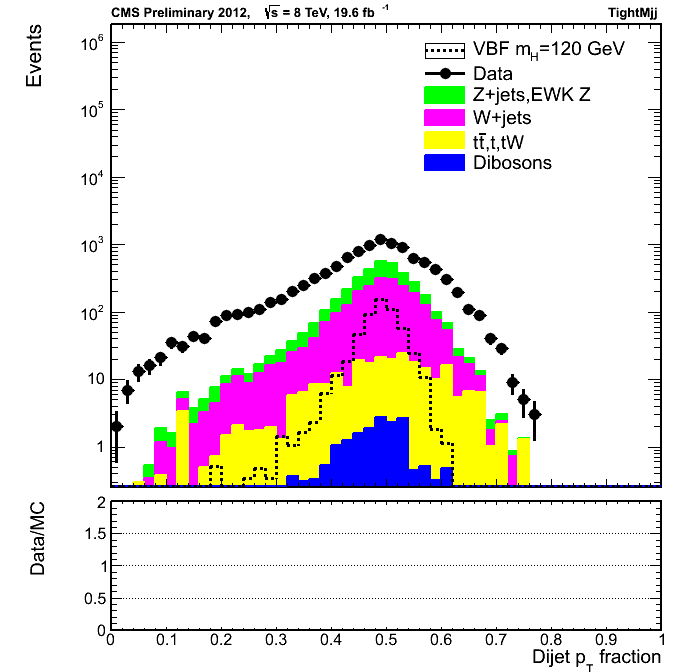
\includegraphics[width=1.00\textwidth]{img/dijetOverMetPt_2012_TightMjj_log.png}
  \end{center}

\end{block}

\column[t]{5.5cm}
\begin{block}{After DijetFraction cut}

  \begin{center}
  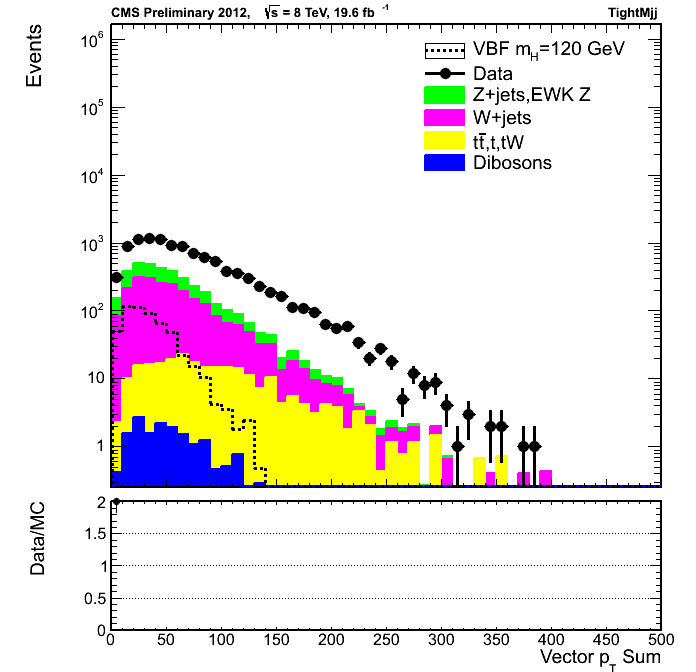
\includegraphics[width=1.00\textwidth]{img/vecSumTriObjectPt_2012_TightMjj_log.png}
  \end{center}

\end{block}
  
\end{columns}
 
\end{frame}

\begin{frame}{2D plots of variables on MC and Data at MET cut level} 
 
\begin{columns}

\column[t]{5.5cm}   
\begin{block}{After MET cut}
 
  \begin{center}
  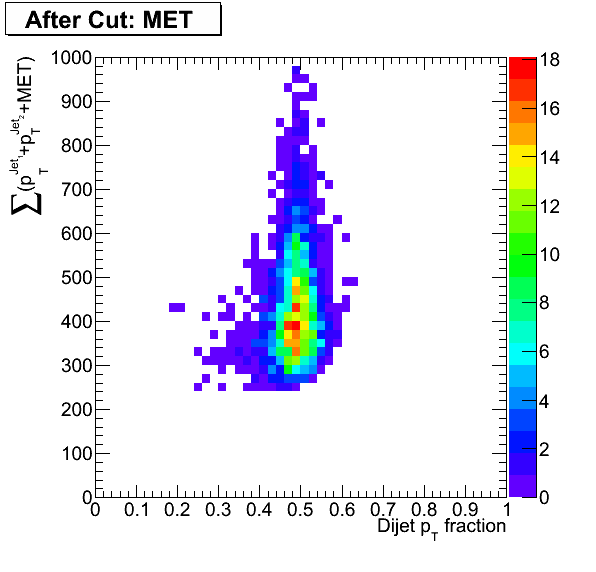
\includegraphics[width=1.00\textwidth]{img/MET_dijetFrac_htMET_VBFInv.png}
  \end{center}

\end{block}

\column[t]{5.5cm}
\begin{block}{After MET cut}

  \begin{center}
  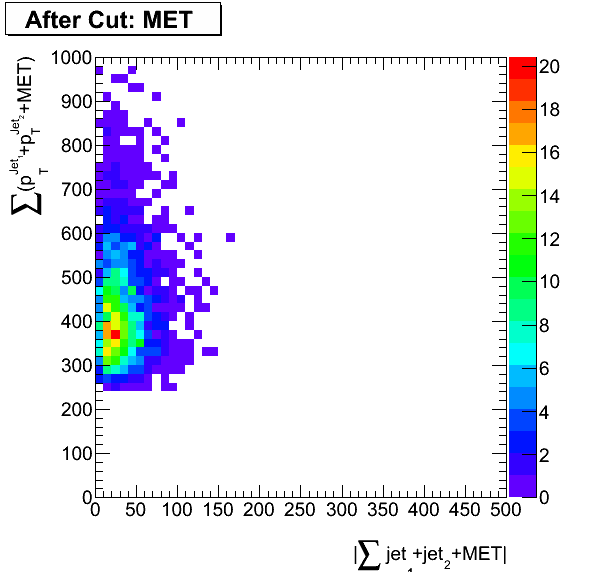
\includegraphics[width=1.00\textwidth]{img/MET_vecSum_htMET_VBFInv.png}
  \end{center}

\end{block}
  
\end{columns}
 
\end{frame}

\begin{frame}{Definition of test cut zones}

\begin{columns}
 

\column[t]{5.5cm}   
\begin{block}{Dijet PT Fraction + scalar pT Sum}
We can define a rectangle cut:
\begin{itemize}
  \item Dijet PT Fraction := [0.46,0.54]
  \item Scalar pT Sum := [250,600]
\end{itemize}

\end{block}

\begin{block}{Vector pT sum + scalar pT Sum}
 We can define a rectangle cut:
\begin{itemize}
  \item Dijet PT Fraction := [0,40]
  \item Scalar pT Sum := [250,550]
\end{itemize}

\end{block}

\end{columns}

\end{frame}

\begin{frame}{Plots before and after cut on $dphi>2.6$ for DijetFrac}

\begin{columns}
  
\column[t]{5.5cm}   
\begin{block}{After TightMjj cut}

  \begin{center}
  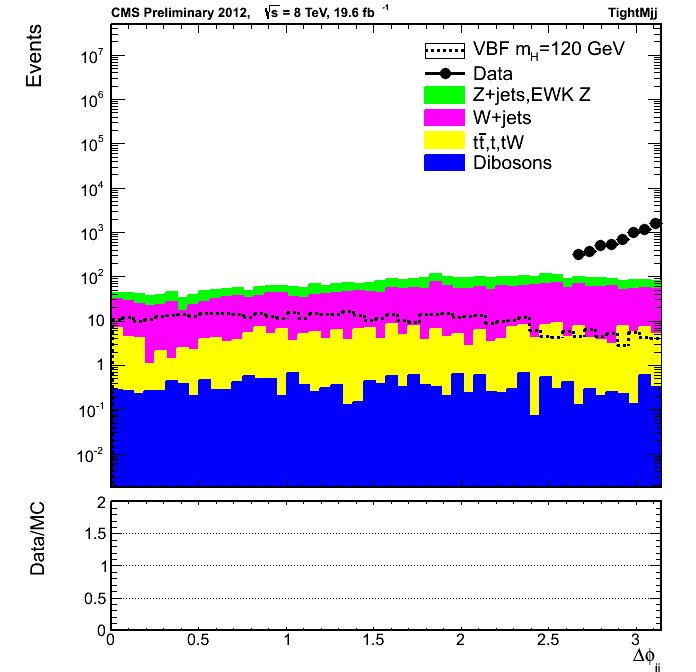
\includegraphics[width=1.00\textwidth]{img/dphijj_2012_TightMjj_log.png}
  \end{center}

\end{block}
  
\column[t]{5.5cm}
\begin{block}{After DijetFraction cut}

  \begin{center}
  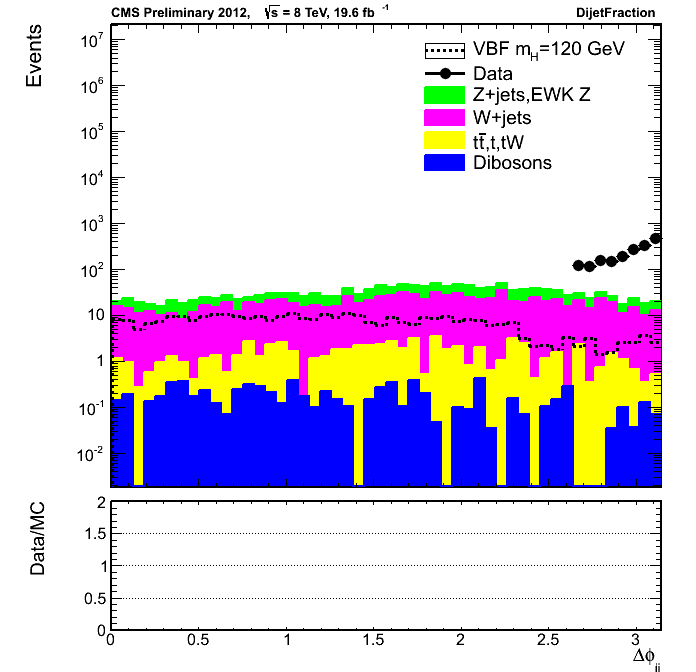
\includegraphics[width=1.00\textwidth]{img/dphijj_2012_DijetFraction_log.png}
  \end{center}

\end{block}
  
\end{columns}
 
\end{frame}

\begin{frame}{Event Yields DijetFraction}

\begin{block}{After TightMjj cut}
  


\begin{tiny}
\begin{center}
  

\hspace*{-1cm}
\begin{tabular}{|l|c|c|c|c|c|c||c|c||c|}
\hline
Step          & QCD                   & W+jets            & Z+jets           & SumMC & Data & Signal 120 \\
\hline
JetPair       & $ 1529141 \pm 103399 $& $ 23443 \pm 107 $ & $ 10769 \pm 51 $ & $ 1571309 \pm 103619 $ & $ 1435063 $ & $ 1440 \pm 21 $ \\ 
AN            & $ 23162 \pm 2055 $    & $ 5192 \pm 60 $   & $ 3534 \pm 32 $  & $ 33018 \pm 2179 $ & $ 32324 $ & $ 856 \pm 18 $ \\ 
DEta          & $ 605071 \pm 46654 $  & $ 11333 \pm 83 $  & $ 5123 \pm 41 $  & $ 623389 \pm 46813 $ & $ 576792 $ & $ 1171 \pm 19 $ \\ 
MET           & $ 8540 \pm 1778 $     & $ 4250 \pm 54 $   & $ 2795 \pm 30 $  & $ 16186 \pm 1885 $ & $ 16282 $ & $ 881 \pm 17 $ \\ 
TightMjj      & $ 6560 \pm 1445 $     & $ 2032 \pm 39 $   & $ 1357 \pm 21 $  & $ 10256 \pm 1521 $ & $ 10481 $ & $ 543 \pm 14 $ \\ 
DijetFraction & $ 3035 \pm 1163 $     & $ 895 \pm 27 $    & $ 584 \pm 14 $   & $ 4606 \pm 1213 $ & $ XXX $ & $ 344 \pm 11 $ \\ 
DPhiSIGNAL    & $ 688 \pm 688 $       & $ 217 \pm 14 $    & $ 130 \pm 7 $    & $ 1057 \pm 714 $ & XXX & $ 137 \pm 7 $ \\ 
DPhiQCD       & $ 2206 \pm 927 $      & $ 129 \pm 10 $    & $ 73 \pm 4 $     & $ 2421 \pm 945 $ & $ 1873 $ & $ 22 \pm 3 $ \\ 
\hline
\end{tabular}
\end{center}

\end{tiny}

\end{block}

\end{frame}

\begin{frame}{Conclusions}
 
\begin{block}{Conclusions}
  
  \begin{itemize}
    \item Variable that use the dijet+MET show signal discrimination potencial for our analysis.
    \item With first attempt of 2D cut, we have a factor of 3 reduction on QCD and keep 60\% of signal.
    \item Vector $p_{T}$ sum, not presented today but similar discrimination is expectable.
  \end{itemize}

\end{block}

\begin{block}{Next}

  \begin{itemize}
    \item Finish Vector $p_{T}$ sum first study
    \item Optimize variables 
    \item Include resolution effects (possible gains)
  \end{itemize}

\end{block}

\end{frame}

\end{document}